\chapter{Technical Background}
\label{sec:state}

% Hier werden zwei wesentliche Aufgaben erledigt:

% 1. Der Leser muß alles beigebracht bekommen, was er zum Verständnis
% der späteren Kapitel braucht. Insbesondere sind in unserem Fach die
% Systemvoraussetzungen zu klären, die man später benutzt. Zulässig ist
% auch, daß man hier auf Tutorials oder Ähnliches verweist, die hier auf
% dem Netz zugänglich sind.

% 2. Es muß klar werden, was anderswo zu diesem Problem gearbeitet
% wird. Insbesondere sollen natürlich die Lücken der anderen klar
% werden. Warum ist die eigene Arbeit, der eigene Ansatz wichtig, um
% hier den Stand der Technik weiterzubringen? Dieses Kapitel wird von
% vielen Lesern übergangen (nicht aber vom Gutachter ;-), auch später
% bei Veröffentlichungen ist "Related Work" eine wichtige Sache.

% Viele Leser stellen dann später fest, daß sie einige der Grundlagen
% doch brauchen und blättern zurück. Deshalb ist es gut,
% Rückwärtsverweise in späteren Kapiteln zu haben, und zwar so, daß man
% die Abschnitte, auf die verwiesen wird, auch für sich lesen
% kann. Diese Kapitel kann relativ lang werden, je größer der Kontext
% der Arbeit, desto länger. Es lohnt sich auch! Den Text kann man unter
% Umständen wiederverwenden, indem man ihn als "Tutorial" zu einem
% Gebiet auch dem Netz zugänglich macht.

% Dadurch gewinnt man manchmal wertvolle Hinweise von Kollegen. Dieses
% Kapitel wird in der Regel zuerst geschrieben und ist das Einfachste
% (oder das Schwerste weil erste).

This chapter will introduce the basic terminology used throughout this work, followed by the related work done in the field of load balancing, and close with a deeper dive into technical concepts reoccurring in Chapter~\ref{sec:design} and Chapter~\ref{sec:implementation}.
Starting with the terminology used throughout this thesis, followed by the related work done in the fields of load balancing and closing with an explanation of the most important topics.

\section{Terminology}

\paragraph{Central Processing Unit (CPU).}
A CPU is the hardware unit that executes an instruction stream.
CPUs or hardware threads are referred to by a logical number, denoted by CPU<N>.

\paragraph{Thread.}
A thread is a schedulable unit of execution.
It contains the state of the execution of a program, like the program counter, stack pointer, and registers, and it is assigned to exactly one CPU at a time.

\paragraph{Virtual CPU (vCPU).}
A vCPU is a kernel abstraction that makes a thread behave like a physical CPU toward the user level.
Events such as interrupts, exceptions, and inter-process communication (IPC, see Section~\ref{sec:ipc}) are delivered asynchronously to a user-level entry point instead of blocking the thread.
It is, therefore, the basis for user-level schedulers and virtual machine monitors.

\paragraph{User-level Thread Control Block (UTCB).}
The User-level Thread Control Block is a small per-thread memory area shared between kernel and user space.
It holds the message registers used for IPC and further thread state that can thus be accessed without a system call.

\paragraph{Floating Point Unit (FPU).}
The FPU is the processor unit for floating-point arithmetic and has its own register set, which forms part of a thread's context. Its state is tracked per CPU and switched either lazily or eagerly.

\paragraph{Components.}
Components are the user-level programs the system is composed of, such as servers, device drivers, and applications.
Each of them runs isolated in its own address space and interacts with the others solely by IPC.

\paragraph{Capability.}
A capability is an unforgeable reference to a kernel or server object, stored in a slot of the task's capability table together with the rights it grants.
A thread can only communicate with objects for which it holds a capability.

\paragraph{Interface.}
An interface is the set of operations an object offers to its clients, invoked via IPC through a capability.
A client only depends on the interface, not on whether the object is implemented in the kernel or in a user-level server.

\paragraph{Proxy.}
A proxy is an object that implements the same interface as another object and forwards invocations to it.
Because clients cannot distinguish it from the original object, it can be interposed transparently to observe, delay, or redirect requests and enforce a policy.

\paragraph{Kernel and User Mode.}
Kernel mode is the privileged processor mode in which the microkernel runs with unrestricted access to the hardware.
All other software runs in the deprivileged user mode.
Crossing this boundary requires a trap into the kernel, making system calls comparatively expensive.

\paragraph{Run Queue.}
The run queue is the per-CPU kernel data structure that holds all threads that are ready to execute, usually ordered by a kind of priority metric.
The scheduler selects the next thread to run from it, which makes its occupancy a direct indicator of the load on that CPU.

\paragraph{Kip Clock.}
The Kernel Info Page (KIP) is a read-only page mapped into every task.
Its clock field contains a monotonically increasing time value in microseconds since boot.
It provides user-level code with timestamps without the cost of a system call at the resolution given by the kernel's timer configuration.

\paragraph{Software Interrupt Requests (IRQ).}
An IRQ object is a kernel object used for asynchronous notification.
A software IRQ is not bound to a hardware source but is triggered by user-level code, which allows one component to signal another without a blocking IPC.

\paragraph{Moe and the In Task Service (ITAS).}
Moe is the root task; it is the first user-level program started by the L4Re microkernel and provides the basic L4Re services such as data spaces, region maps, and name spaces.
ITAS is the event handler thread that is loaded into every application's address space, where it acts as a region manager, pager, and exception handler for that application.

\section{Related Work}

\subsection{General Purpose Scheduling}

This section will cover the Linux and Windows as representatives for general purpose scheduling in monolithic operating systems.
The Linux completely fair scheduler (CFS) and its successor, earliest eligible virtual deadline first (EEVDF), share the same load-balancing strategy, as their differences are located in core local scheduling decisions.
The utilization of a CPU is determined by the threads and thread groups located on that CPU via per-entity load tracking (PELT)~\cite{linux-internals-loadbalancing}.
Load balancing is triggered periodically, on idle CPUs and on thread wake/create events.
Linux employs scheduling domains that are then balanced by one designated CPU that can migrate up to 32 threads at a time between the busiest and idlest scheduling groups.
The domains are organized in a topology that is balanced from the bottom up.
Additionally, imbalance thresholds scaling with distance and cache-locality heuristics are used on non-uniform memory access (NUMA) systems, limiting unnecessary migrations~\cite{wasted_cores, cfs_vs_ule}.

Windows follows a pull-based approach where idle processors search for work and try to steal it instead of busy ones pushing it away.
In contrast to Linux, no periodic rebalancing is executed, but rather on-demand when the placement logic finds a better CPU.
The thread placement employs a hierarchical fallback order based on simultaneous multithreading (SMT) topology: ideal (assigned at thread creation time), last, current, same-SMT-set, and lowest-numbered CPU to preserve cache locality.
NUMA and SMT awareness are provided by proactive migrations at the quantum end when a thread's SMT set is busy while ideal nodes remain idle~\cite{windows_internals, clr_inside_out}.

Both designs are mechanism-rich with the advantage of having all scheduling information without any overhead because of the monolithic operating system design.
The microkernel philosophy prohibits such behavior, as a load balancer residing in userland cannot have detailed information about the whole system state right away but needs to obtain it from the kernel via a dedicated interface.

\subsection{AMP Aware Load Balancing}

Asymmetric multiprocessing (AMP) awareness describes the ability of a balancing system to have knowledge about the processor architecture underneath and use it to make informed decisions.
The work of Li \textit{et al.}~\cite{faster-core-first} extended the Linux CFS with AMPS to harness asymmetric multi-core architectures (see Section~\ref{sec:amp}).
To overcome the differences in performance and efficiency cores, they presented three concepts.
First, scaling the CPU load by its compute power, populating fast cores first, a policy known as \enquote{faster core first}; and finally, gating migrations by NUMA and cache-miss cost prediction.
Although a minimal patch to CFS, it still sits on top of a monolithic scheduler, contrasting a from-scratch design followed through in this thesis.

Shelepov and Saez \textit{et al.}~\cite{hass-scheduling} took an offline approach with Heterogeneous Awareness Scheduling (HASS) on OpenSolaris, avoiding runtime overhead entirely by matching threads to core types via architectural signatures collected in advance and used to predict per-core completion time.
HASS achieves performance comparable to an omniscient static assignment, but the reliance on offline profiling means it cannot react to shared-cache contention or a thread's phase changes at runtime.
The authors previously explored a dynamic load-balancing approach but found that HASS's offline profiling outperformed it.
The static-vs-dynamic trade-off this exposes is directly relevant to a design that instead derives its load signal from the kernel's own runtime state.

Koufaty, Reddy, and Hahn~\cite{bias-scheduling} took a lighter-weight, fully online approach with bias scheduling, classifying each thread's preference for big or small cores from internal versus external stall counters already present in hardware.
They apply the classification only at the point of load balancing rather than continuously.
Their evaluation is notable for modeling heterogeneity through distinct core microarchitectures rather than the frequency-scaled cores common in earlier work.
Additionally, they show that DVFS-based emulation of heterogeneity produces significantly different behavior from real asymmetric cores.
The low-overhead, existing-counter-based metric is conceptually close to the online concepts used in this thesis, even though bias scheduling still classifies threads only coarsely rather than estimating cross-core performance directly.

Van Craeynest \textit{et al.}~\cite{pie} pushed the estimation further with Performance Impact Estimation (PIE), predicting cross-core performance from a thread's cycles per instruction stack together with its memory- and instruction-level parallelism rather than sampling actual execution on the other core type.
PIE improves prediction accuracy over both sampling- and bias-based approaches at a hardware cost the authors report as roughly 15 bytes of additional per-core hardware state, but this comes at the price of a considerably more elaborate estimation model.
Where PIE trades metric simplicity for prediction accuracy, this thesis takes the opposite position, favoring a simple, directly observable metric over a modeled estimate of cross-core performance.

\subsection{Microkernel Load Balancing}

QNX's AMP support forgoes runtime load balancing altogether: CPU-to-process binding is fixed at boot time, and the vendor documentation explicitly characterizes dynamic migration as impractical given the cost of checkpointing and interrupting a running process~\cite{qnx-amp}.
Notably, QNX's use of the term \enquote{AMP} differs from the hybrid-core sense used in this thesis, as it also covers configurations running entirely different operating systems per core rather than cores of a single ISA with different performance characteristics.
QNX, therefore, represents something close to a null case among the related work, showing the motivation for a dynamic, AMP-aware balancer in a microkernel setting.

The seL4-derived balancer described in~\cite{global-dynamic-load-balancing} is one of the few load-balancing designs implemented directly for a microkernel rather than retrofitted onto a monolithic scheduler.
It follows a centralized design in which load is computed as the summed remaining time slices of ready threads per core and compared against a static twenty percent imbalance threshold, with rebalancing triggered both on thread creation and by a 100\,\si{\ms} periodic timer, migrating a thread only if doing so strictly improves the balance.
The design has seen limited adoption or follow-up, targets homogeneous microkernel cores exclusively, and does not address asymmetric hardware, leaving open the exact gap this thesis addresses.

\subsection{L4Re Implementations}

In 2013 Kuang, Waddington, and Tian~\cite{omnire} diagnosed L4Re's poor scalability on Fiasco.OC at 48 cores to a single-threaded Sigma0 pager.
Additionally, it was found that overhead for cross-core IPC is roughly an order of magnitude higher than same-core IPC.
This gap is addressed with OmniRE, a decentralized personality that gives each core its own resource-managing Omni-Core and App-Cores rather than routing through a single system-wide pager.
OmniRE outperforms vanilla L4Re at high core counts and can exceed Linux in memory page management, demonstrating the benefit of localizing resource management to individual cores rather than centralizing it.
The work targets SMP scalability rather than AMP awareness, but its core localization principle directly motivates minimizing cross-core migrations.

Eppelt's thesis~\cite{philipp-thesis}, produced at the same chair, is a direct predecessor to this work: a user-level load balancer for the L4Re microkernel that reads hardware performance counters and combines them with a static per-task configuration.
The developed system aggregates observed data in a measure-predict-decide-enforce cycle, evaluating four balancing algorithms against Linux's CFS on a homogeneous Haswell SMT system.
The results show CFS ahead on raw throughput, whereas the behavior-aware algorithms achieve better fairness and lower deviation between cores rather than higher speed.
Eppelt explicitly identifies heterogeneous AMP hardware as future work outside the scope of that thesis, which is precisely the continuation this work undertakes, and his framing of fairness as a benefit distinct from throughput is one this thesis picks up again.

\section{Microkernel-Based Operating Systems}

Microkernel architectures follow a minimalist design philosophy.
The kernel is reduced to a small set of essential services that are strictly required to implement the foundational tasks of an operating system.
Everything else, with the possible exception of CPU scheduling for performance reasons, is executed in user space.
Components that introduce any kind of policy, such as file systems, drivers, or the networking stack, are thus implemented as separate user space services and can be tailored to the needs of the system or omitted entirely.
This modularization improves fault isolation and system robustness, as failures in individual components do not compromise the kernel~\cite{core-dumps, IntroMOSlecture}.

\subsection{L4Re Operating System Framework}

L4Re~\cite{l4re} consists of two parts: the microkernel, called Fiasco, and a collection of userland components.
It adheres to the microkernel philosophy of keeping the kernel free of policy and pushing all strategies and decisions into userland components.
This modular approach allows for a wide range of use cases in the embedded, real-time, hypervisor, and secure computing domains while maintaining strict isolation between components.
To help enforce those constraints in practice, a mechanism is needed that allows userland components to transparently intercept and extend kernel-provided primitives without the application being aware of it.

\paragraph{Proxy Pattern.}
\label{sec:proxy}

In L4Re the proxy pattern is a design used to allow for flexible modularization and layered components that each enforce their own policy.
A proxy service implements the interface of the component it embodies.
It can then be handed to an application that cannot distinguish between the original kernel primitive and the proxy acting as an intermediate layer enforcing a policy.
This pattern exposes interfaces in a structured manner, which is especially important when impersonating the kernel application programming interface (API).

\section{Information Exchange}

Because of the isolation inherent to a microkernel-based operating system, applications require mechanisms to communicate with each other and with the kernel to coordinate their actions.
To communicate with the kernel, system calls are used.
There are two main concepts to address userland communication, although the fact that the target hardware is a multi-core system introduces additional variations.

\paragraph{Inter-Process Communication}
\label{sec:ipc}

In L4Re inter-process communication (IPC) provides a means of message passing in a synchronous fashion.
Both partners need to meet at a rendezvous point in time to exchange information.
The sender and receiver must block for each other while data is copied once from one partner to the other via the UTCB~\cite{IPCMOSlecture}.
Because the UTCB is limited in size, this communication channel does not allow for arbitrary memory exchanges within one call.

\paragraph{Shared Memory}

An asynchronous alternative is shared memory, which relies solely on both partners having access to the same region of memory.
This allows them to read from or write to this region at arbitrary times without waiting for their partner~\cite{IPCMOSlecture}.

\paragraph{Cross-Core Communication}
\label{sec:cross-comm}

When communication needs to cross the boundary of a CPU, delivery of an incoming IPC message is handled through an inter-processor interrupt (IPI).
Broken down, an IPC message on the same CPU is a context switch from one thread to another.
An IPI interrupts the current execution on the destination CPU for a short period until the interrupt has been handled, leading to a cross-core context switch.
IPIs are comparatively expensive in hardware.
If a CPU is flooded with IPIs, threads scheduled on it can experience a significant slowdown, so the excessive use of IPIs should be avoided.
IPC also provides the mechanism of a deferred request (DRQ) that hands a request from the sender to the thread that is meant to execute it.
The target thread then uses its own priority on its own CPU to execute the job and reply to the sender, which remains blocked for the duration.

\section{CPU Scheduling}

The CPU is a shared resource, so scheduling policies are required to determine which thread is granted execution time.
In multitasking systems, scheduling is usually done preemptively.
The currently executing thread is interrupted regularly so that the operating system can retake control of the CPU~\cite{ostep}.
The scheduling policy in use determines which thread is chosen next for execution.
A simple but effective strategy is to always choose the thread with the highest assigned priority, a policy known as priority-based scheduling.
The moment a thread of higher priority becomes ready to run, the scheduler elects that thread to run immediately and suspends the previously running one.
Priorities can be assigned in a static or dynamic fashion depending on the strategy.
L4Re employs this policy at runtime and additionally uses round-robin scheduling for threads that share the same priority~\cite{rr-scheduling}.

\subsection{Best-Effort Scheduling}
\label{sec:best-effort}

Policies belonging to this class attempt to have all threads in the system finish as quickly as possible without providing any guarantee on when or in what order a given thread will complete.
Instead of enforcing hard timing constraints, best-effort schedulers optimize for objectives such as fairness, system throughput, low average response time, or energy efficiency~\cite{ostep}.
Established best-effort schedulers such as Linux's Completely Fair Scheduler and its successor, the Earliest Eligible Virtual Deadline First scheduler, approximate fairness by tracking the virtual runtime each thread has already received and preferring threads that have run the least~\cite{cfs, eevdf}.
Real-time systems, in contrast, additionally require threads to meet explicit deadlines, which best-effort scheduling alone cannot guarantee.

\section{Load Balancing}

On a multiprocessor system, each CPU typically executes its own local scheduling policy and makes decisions independently of the other CPUs in the system.
Left unmanaged, this can lead to an uneven distribution of work.
Load balancing addresses this by redistributing threads across CPUs so that the system as a whole approaches a chosen optimization goal, complementing rather than replacing the local scheduling policy on each CPU.
System requirements dictate for which goal should be optimized for.
In modern systems, this ranges from maximizing throughput and minimizing average response time to meeting deadlines and providing deterministic timing guarantees~\cite{load-balancing}.
Any such policy first requires a notion of load, a metric that quantifies how much demand a CPU is currently facing, before CPUs can meaningfully be compared and classified as overloaded or underloaded.

\subsection{Strategies}

A load-balancing strategy is an algorithm that determines on which CPU a thread should execute.
This decision can be triggered by various events, for example, when a CPU becomes overloaded, a thread is newly created, or a thread experiences degraded performance.
Such strategies are commonly grouped into three categories: partitioned, global, and semi-partitioned scheduling~\cite{acm-loadbalancing-algos}.
In partitioned scheduling, each thread is assigned to exactly one CPU for its entire lifetime, so migrations never occur.
This avoids migration overhead entirely, but finding an assignment that keeps every CPU evenly loaded is equivalent to a bin-packing problem and is known to be NP-hard in the general case~\cite{semi-np-hardness}.
Global scheduling instead treats all CPUs as a shared pool, so any ready thread may, in principle, execute on any CPU, and threads may migrate freely between CPUs.
This allows the load to be distributed far more evenly, at the cost of migration overhead and reduced cache locality whenever a thread is moved.
Semi-partitioned scheduling combines both approaches, keeping most threads statically bound to a CPU while allowing a smaller subset to migrate so as to balance out remaining imbalances, trading the simplicity of partitioning for better utilization.

\subsection{Approaches}
\label{sec:approaches}

For employing either a global or a semi-partitioned balancing policy, one of three approaches can be used.
They differ mainly in where the decision to migrate a thread is made and how much information about the rest of the system is required.

\paragraph{Push.}

The moment a CPU detects that it is overloaded, it can try to offload work to other CPUs.
Because the decision originates from the overloaded CPU itself, only local information about that CPU's own state is strictly required, although knowledge of at least one suitable target CPU is still needed to decide where to push work.

\paragraph{Pull.}

When a CPU has spare capacity or runs idle entirely, it can pull work from other CPUs onto its own run queue and thereby reduce the pressure elsewhere in the system.
A well-known instance of this approach is work stealing, where an idle CPU actively looks for a busy one to take work from rather than waiting for work to be pushed to it.

\paragraph{Centralized.}

A third method is to have a centralized instance monitor all CPUs and redistribute work as soon as overloaded or underloaded CPUs are detected.
This approach can make more globally informed decisions than push or pull, as it has visibility into the state of every CPU at once, but it introduces a single component whose own overhead and responsiveness directly affect how well the system as a whole is balanced.

\section{Asymmetric Multi-Processing}
\label{sec:amp}

Modern computers have moved away from uniform CPUs with identical characteristics toward systems built from CPUs of different types with deviating attributes.
This technique is referred to as asymmetric multiprocessing (AMP).
Examples of this asymmetric multi-core architecture include ARM's big.LITTLE~\cite{arm_big_little_2026}, AMD's Zen~\cite{amd_zen_core_2026}, and Intel's hybrid architectures~\cite{intel_hybrid_architecture_2026}.
By combining high-performance cores optimized for compute-intensive workloads with energy-efficient cores designed for lighter background tasks, these designs aim to provide hardware that is better suited to the mix of workloads found in typical systems than a uniform design would be.
An example socket with two performance and four efficiency cores can be seen in Figure~\ref{fig:hetero-cpu-arch}.

\begin{figure}[h]
	\centering
	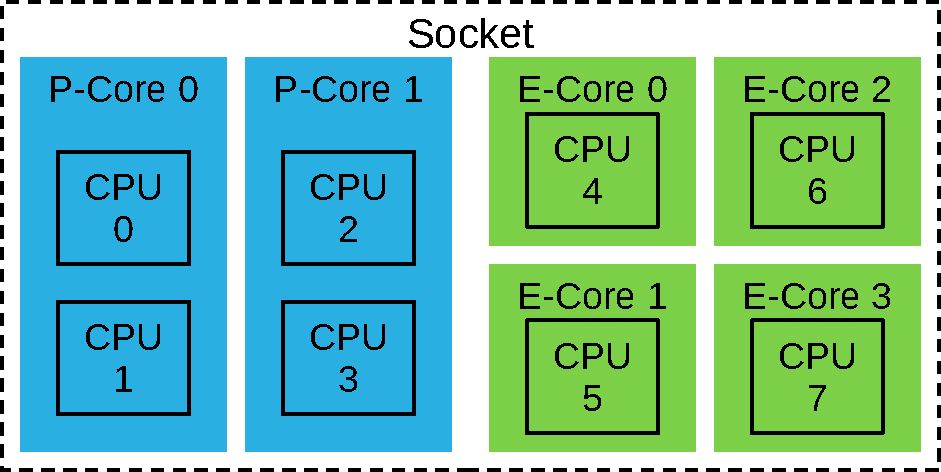
\includegraphics[width=0.65\linewidth]{images/heterogeneous_cpu_arch.pdf}
	\caption{Heterogeneous CPU architecture with two P-cores housing two hardware threads each and four E-cores with one CPU each on a single socket.}
	\label{fig:hetero-cpu-arch}
\end{figure}

For an operating system, this heterogeneity means that CPU time can no longer be treated as an interchangeable resource because the same workload can be completed in a different amount of time depending on which core type it is scheduled on.
This fact needs to be accounted for by any load-balancing policy targeting such hardware when trying to optimize for its given goal.

\subsection{Heterogeneous CPU Architecture}
\label{sec:hetero-cpu-arch}

Not only has the compute power of individual CPUs changed, but the physical placement of hardware threads has also moved from a uniform to a heterogeneous design.
Performance cores commonly combine multiple hardware threads onto a single physical core through SMT and share resources such as caches between them.
Efficiency cores typically retain a single hardware thread per core but are grouped into clusters that share a last-level cache among several cores (see Figure~\ref{fig:hetero-cpu-arch}).
One example of this architecture is the Intel Core i9-13900K Processor, \footnote{\href{https://www.intel.com/content/www/us/en/products/sku/230496/intel-core-i913900k-processor-36m-cache-up-to-5-80-ghz/specifications.html}{Intel Core i9-13900K Processor Specification}} used as testing hardware in this work.
This layout means that two hardware threads considered equally available by the operating system can in practice compete for the same shared cache, so a scheduler that is unaware of this topology risks placing threads in a way that looks balanced on paper but causes contention in hardware.

\cleardoublepage

%%% Local Variables:
%%% TeX-master: "diplom"
%%% End:
